\def\g#1{{\color{gray}{#1}}}

\lecture{Máximo Divisor Comum -- MDC}{mdc}
\frame{\title{\insertlecture}\maketitle}

\section{\insertlecture}

\begin{frame}{Máximo divisor comum -- MDC}

  Assuma que $D$, $P$, $Q$ sejam inteiros positivos.\\
  \bigskip
  $D$ divide $P$ significa $D\div P$ é um número inteiro.\\
  \bigskip
  O {\bf maior divisor comum}  de $P$ e $Q$ -- escrito $MDC(P, Q)$ --
  é o maior número que divide $P$ e $Q$.
  \bigskip
  
  \onslide<2>
  Exemplo:\\
  \bigskip
  Divisores de 18: {\small $1\ 2\ \g{3}\ \g{4}\ \g{5}\ 6\ \g{7}\ \g{8}\ 9\
    \g{10}\ \g{11}\ \g{12}\ \g{13}\ \g{14}\ \g{15}\ \g{16}\ \g{17}$}\\
\bigskip
  Divisores de 12: {\small $1\ 2\ 3\ 4\ \g{5}\ 6\ \g{7}\ \g{8}\ \g{9}\
    \g{10}\ \g{11}\ \g{12}$}\\
    
\end{frame}

\begin{frame}{Alguns fatos sobre MDC}
  
\only<1->{{\color<2->{gray}
    Teorema: $MDC(P,Q)$ igual a $MDC(Q,P)$.\\
  }}
\bigskip
\only<2->{{\color<3->{gray}
    Teorema: $MDC(P, P)$ igual a $P$.\\
  }}
\bigskip
\only<3->{
  \begin{tabbing}
    Teorema: \= If $P$ é menor que $Q$ então\\
    \> $MDC(P,Q)$ é igual a $MDC(P, Q-P)$
  \end{tabbing}
}
\end{frame}


\begin{frame}{Algoritmo de Euclides}
  
  \begin{itemize}
  \item Descrito pelo matemático grego Euclides nos livros VII e X de
    ``Elementos'', por volta do ano 300 AC;
  \item Um dos algoritmos numéricos mais antigos ainda em uso;
  \item Uma das aplicações do algoritmo é servir como base para o
    algoritmo criptográfico RSA\footnote{Rivest, Shamir e Adleman},
    amplamente utilizado no comércio eletrônico.
  \end{itemize}

\end{frame}

\def\y{1cm}
\begin{frame}{Ideia básica do algoritmo de Euclides}
  
  \begin{tikzpicture}[every node/.style={anchor=west}]

  
    \node<1-> (s0) at (0,5*\y) {\color<2->{gray}{Computar o $MDC(M,N)$ para inteiros positivos $M$, $N$:}};
    
    \node<2-> (s1) at (0,4*\y) {\color<3->{gray}{Usando as variáveis $x$ e $y$.}};
    
    \node<3-> (s2) at (0,3*\y) {Mantendo verdade {\color{blue}{$MDC(x,y)=MDC(M,N)$}} (a invariante)};
    \node<9>[draw,minimum width=10.75cm,minimum height=1cm] at (0,3*\y) {};

    \node<4-> (s3) at (0,2*\y) {A computação para ({\em halt}) quando $x$ é igual a $y$};
    \node<8>[draw,minimum width=8.5cm,minimum height=1cm] at (0,2*\y) {};

    \node<5->[] (s4) at (\y,\y) {{\bf Teorema: } $MDC(x,x)$ é igual a $x$.};
    \node<7>[draw,minimum width=6.5cm,minimum height=1cm] at (\y,\y) {};

    \node<6->[text=blue] (s4) at (0,0) {Quando parar:};
    \node<8>[draw,minimum width=3cm,minimum height=1cm] at (0,0) {};

    \node<7->[text=blue] at (0,-1) {{\color<8->{blue!30}$x$ é igual\ }\color<8>{blue}{\color<9->{blue!30} $MDC(x,x)$ \only<8->{é igual a\ }}
      \only<8->{\color<9->{blue} $MDC(x,y)$} \only<9->{\color{blue} é igual a $MCD(M,N)$}};

\end{tikzpicture}

\end{frame}

\begin{frame}{Descrevendo o algoritmo de Euclides com matemática}

  \begin{tikzpicture}
    
    \node<1-> (init) {\color<2->{gray}$Init_{euclides}$: \color<1>{blue} $(x=M) \wedge (y=N)$};
    \node<2->[] (next) [below of=init] {\color<3->{gray}$Next_{euclides}$: 
      \only<4->{\color<4>{blue} \color<5->{blue!30} $((x<y)\wedge(x^\prime=x)\wedge(y^\prime=y-x))$}};

    \node<6>[] [below of=next,xshift=1cm,yshift=.45cm] {\color{blue} $\vee((y<x)\wedge(y^\prime=y)\wedge(x^\prime=x-y))$};

    \node<1->[anchor=west] (truth) [below of=init,yshift=-1.5cm]  {\color<2->{gray} Manter a verdade {\color<1>{blue}$MDC(x,y)=MDC(M,N)$} (a invariante)};
    \node<2->[anchor=east] (nexti) [below of=truth] {\color<3->{gray}Assegurar que $Next_{euclides}$ implica em {\color<2>{blue} $MDC(x^\prime, y^\prime)=MCD(x,y)$}};

    \node<3->[anchor=east] (theorem) [below of=nexti] {Usar o {\bf Teorema}: Se \only<3,4>{$x$}\only<5->{$y$} 
      é menor que \only<3,4>{$y$} \only<5->{$x$}  então};
    \node<3-> [below of=theorem,xshift=2.25cm,yshift=.275cm] {\only<3,4>{$MDC(x,y)=MDC(x,y-x)$} \only<5->{$MDC(y,x)=MDC(y,x-y)$}};

  \end{tikzpicture}
  
\end{frame}

\def\M{{\color{red}18}}
\def\N{{\color{brown}12}}
\def\dx{2.25cm}
\def\dy{-1.5cm}
\begin{frame}{Descrevendo o algoritmo de Euclides com matemática}

  \begin{tikzpicture}[every node/.style={anchor=west}]
    
    \node<1,15>  at (0,0) {$Init_{euclides}:$ \color{blue} $(x=M) \wedge (y=N)$};
    \node<2-14> at (0,0) {$Init_{euclides}:$ \color{blue} $(x=\M) \wedge (y=\N)$};

    \node<1->[] at (0,\dy) {\color<2-3>{gray}$Next_{euclides}$:}; 
    \node<1-3,15>[text=blue] at (\dx, \dy) {\color<2-3>{blue!30} $((x<y)\wedge(x^\prime=x)\wedge(y^\prime=y-x))$};
    \node<1-3,15>[text=blue] at (\dx, 1.5*\dy) {\color<2-3>{blue!30} $\vee((y<x)\wedge(y^\prime=y)\wedge(x^\prime=x-y))$};
    
    \node<4>[] at (\dx, \dy) {\color{blue} ${((\M<\N)}\wedge(x^\prime=\N)\wedge(y^\prime=\N-\M))$};
    \node<4,5>[] at (\dx, 1.5*\dy) {\color{blue} $\vee((\N<\M)\wedge(y^\prime=\N)\wedge(x^\prime=\M-\N))$};

    \node<5>[] at (\dx, \dy) {\color{gray!80} ${((18<12)}\wedge(x^\prime=12)\wedge(y^\prime=12-18))$};
    \node<5>[red,minimum width=2cm, draw] at (\dx,\dy) {FALSA};

    \node<6>[red,minimum width=6cm, draw] at (\dx,\dy) {FALSA};
    \node<6>[] at (\dx, 1.5*\dy) {\color{blue} $\vee(VERDADEIRA\wedge(y^\prime=12)\wedge(x^\prime=6))$};

    \def\M{{\color{red}6}}
    \def\N{{\color{brown}12}}

    \node<7>[text=blue] at (\dx, \dy) {\color<7>{blue} $((\M<\N)\wedge(x^\prime=x)\wedge(y^\prime=\N-\M))$};
    \node<7,8>[text=blue] at (\dx, 1.5*\dy) {\color<7>{blue} \color<8>{gray} $\vee((\N<\M)\wedge(y^\prime=\N)\wedge(x^\prime=\M-\N))$};

    \def\M{{\color{red}6}}
    \def\N{{\color{brown}6}}
    \node<8,9>[text=blue] at (\dx, \dy) {\color{blue} $(VERDADEIRA\wedge(x^\prime=\M)\wedge(y^\prime=\N))$};
    \node<8>[red,minimum width=2cm, draw] at (1.25*\dx,1.5*\dy) {FALSA};

    \node<9>[red,minimum width=6cm, draw] at (1.25*\dx,1.5*\dy) {FALSA};

    \node<10,11>[] at (\dx, \dy) {\color{blue}\color<11>{gray} ${((\M<\N)}\wedge(x^\prime=\N)\wedge(y^\prime=\N-\M))$};
    \node<10,11>[] at (\dx, 1.5*\dy) {\color{blue}\color<11>{gray} $\vee((\N<\M)\wedge(y^\prime=\N)\wedge(x^\prime=\M-\N))$};
    
    \node<11>[red,minimum width=2cm, draw] at (\dx,\dy) {FALSA};
    \node<11>[red,minimum width=2cm, draw] at (1.25*\dx,1.5*\dy) {FALSA};
    
    \node<12-14>[red,minimum width=6cm, draw] at (\dx,\dy) {FALSA};
    \node<12-14>[blue] at (\dx,1.5*\dy) {$\vee$};
    \node<12-14>[red,minimum width=6cm, draw] at (1.25*\dx,1.5*\dy) {FALSA};

    \node<13-14>[red] at (0, 2.5*\dy) {\color<14>{gray}Não há próximo estado!};

    \node<14-15>[red] at (0, 3*\dy) {A computação para ({\em halts}) quando {\color{blue}x} é igual a {\color{blue}y}.};

    \node<15>[red] at (2.5*\dx, 4*\dy) {\color{blue} MDC(18,12)=6};

    \node<1,2>  at (0,2.5*\dy) {\color<2>{gray}Vamos testar com 
      {\color{red}M} igual a {\color{red} 18} e {\color{brown}N} igual a {\color{brown} 12}.};
    
  \node<2-3>[font=\small]  at (0,3*\dy) {A condição inicial determina o primeiro estado da computação.};
  \node<3>[text width=11cm,font=\small] at (0,3.5*\dy) {Para acharmos o próximo ({\em Next}) estado da computação, 
    substituímos $x$ e $y$ na fórmula dos próximos estados possíveis.)};

  \node<2-> at (0,4.5*\dy) {$x=${\color{red}18}, $y=${\color{brown}12}\only<6->{ $\rightarrow$ $x=6, y=12$} 
    \only<9->{ $\rightarrow$  $x=6, y=6$}};

  
\end{tikzpicture}

\end{frame}


\begin{frame}{Descrevendo o algoritmo de Euclides com matemática}
  \begin{tikzpicture}[every node/.style={anchor=west}]
    
    \node  at (0,0) {$Init_{euclides}:$ \color{blue} $(x=M) \wedge (y=N)$};

    \node at (0,\dy) {\color<2-3>{gray}$Next_{euclides}$:}; 
    \node[text=blue] at (\dx, \dy) {$((x<y)\wedge(x^\prime=x)\wedge(y^\prime=y-x))$};
    \node[text=blue] at (\dx, 1.5*\dy) {$\vee((y<x)\wedge(y^\prime=y)\wedge(x^\prime=x-y))$};
    
    \node[text width=11cm] at (0, 2.25*\dy) {Derivamos o algoritmo de tal forma que ele 
    mantenha o estado verdadeiro em cada passo da computação:};
  
  \node at (\dx,3*\dy) {$Inv_{euclides}:$ \color{blue} MDC(x,y)=MDC(M,N)};

  \node at (0,3.75*\dy) {Assegurando que $Init_{euclides}$ {\color{blue}implica} $Inv_{euclides}$};
  
  \node at (\dx,4.5*\dy) {$Inv_{euclides} \wedge Next_{euclides}$ {\color{blue}implica} $Inv_{euclides}^\prime$}; 

  \end{tikzpicture}
\end{frame}

\begin{frame}{MDC}{Especificação completa}

  GCD - {\em Greatest Common Divisor}\\ {\tiny A expressão
    $PositiveInteger$ siginifica que qualquer número Natural pode ser
    escolhido desde que seja diferente de $0$. {\sc theorem} pode ser
    ignorado, por enquanto, para nosso propósito.}

  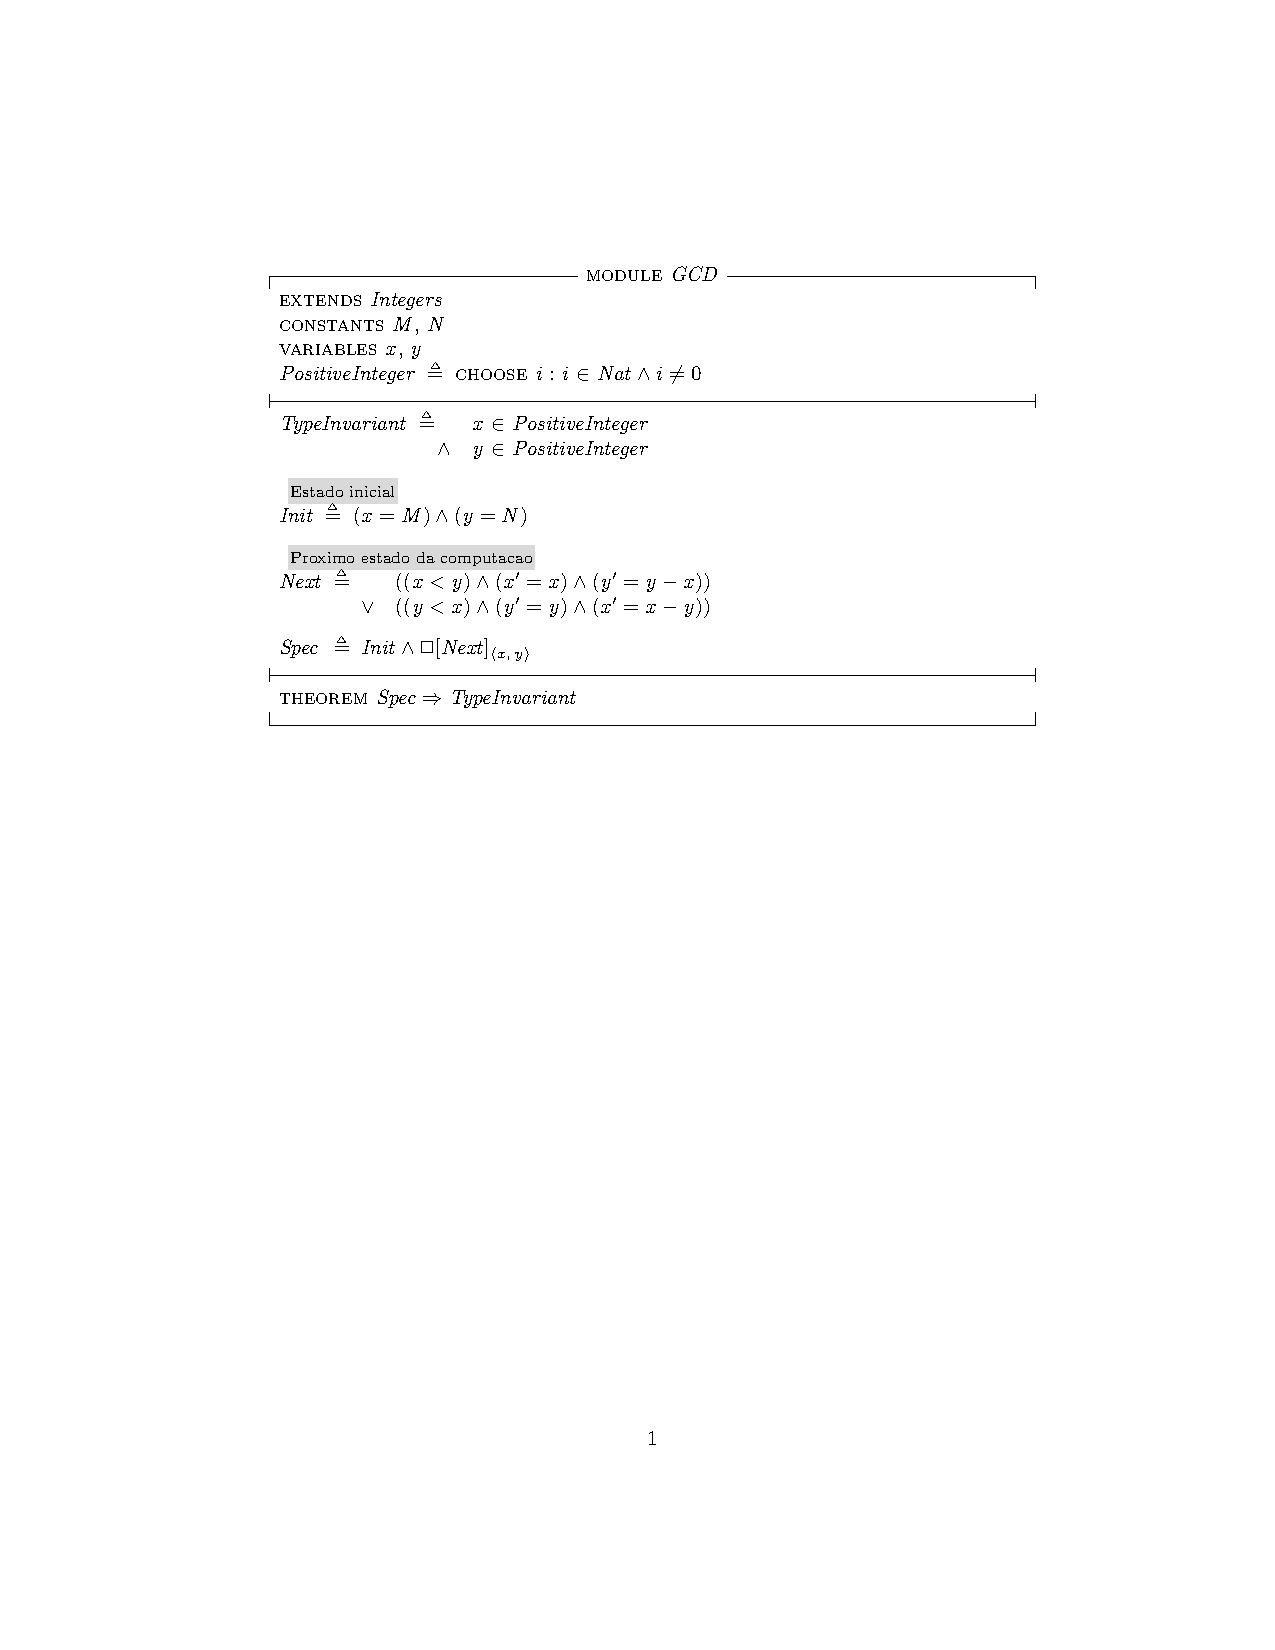
\includegraphics[scale=.5]{../src/GCD.pdf}

\end{frame}

\begin{frame}{Referências}
 
  \begin{enumerate}
  \item \href{http://www.youtube.com/watch?v=BDPHfRuAFnU}{What is
      Computation?} Leslie Lamport, Microsoft, 2011.
    
  \end{enumerate}
  
\end{frame}

